\section*{Results}
% Figures -> Confusion matrices and Heat Maps
% answers “what?”

\subsection*{Arabic Results}
\begin{center}
 \begin{tabular}{c c c c c c c}
     %\hline
     \toprule
     \small{\#                    }& 
     \small{data size    }& 
     \small{encoding     }&
     \small{diacritic    }&
     \small{archit.      }&
     \small{f1           }     \\
     %\hline
     \midrule
    % NOTE: make the expressions full data, eliminated, .. so clear and link them
    % to the model section.

% NOTE:  +1 add to the layer number
% NOTE:  see a way to add the architecture details for each model.

   %  relearn_drop_2_Exp_6_full_data_matrix_with_tashkeel_two_hot_encoding_Bidirectional_LSTM_6_50_0
   \small{1} & \small{full data} & \small{two-hot} & \small{Yes} & \small{7L, 50U, 1} &\small{95.79\%}\\ 
   % relearn_drop_2_Exp_5_full_data_matrix_without_tashkeel_two_hot_encoding_Bidirectional_LSTM_6_50_0
   \small{2} & \small{full data} & \small{two-hot} & \small{No} & \small{7L, 50U, 0} & \small{95.43\%}\\ 
   % relearn_drop_2_Exp_7_full_data_matrix_with_tashkeel_8bitsEncoding_Bidirectional_LSTM_6_81_0
   \small{3} & \small{full data} & \small{binary} & \small{Yes} & \small{7L, 81U, 0} & \small{95.51\%}\\ 
   % relearn_drop_2_Exp_7_full_data_matrix_without_tashkeel_8bitsEncoding_Bidirectional_LSTM_9_30_0
   \small{4} & \small{full data} & \small{binary} & \small{No} & \small{10L, 81U, 0} & \small{93.2\%}\\ 
   % relearn_drop_2_Exp_6_full_data_matrix_with_tashkeel_one_hot_encoding_Bidirectional_LSTM_6_50_1
   \small{5} & \small{full data} & \small{one-hot} & \small{Yes} & \small{7L, 50U, 1} & \small{95.32\%}\\ 
   % relearn_drop_2_Exp_1_full_data_matrix_without_tashkeel_one_hot_encoding_Bidirectional_LSTM_3_50_0
   \small{6} & \small{full data} & \small{one-hot} & \small{No}  &\small{7L, 82U, 0} & \small{93.94\%}\\ 
   % relearn_drop_2_Exp_8_eliminated_data_matrix_with_tashkeel_two_hot_encoding_Bidirectional_LSTM_6_81_1/
   \small{7} & \small{eliminated} & \small{two-hot} & \small{Yes} & \small{7L, 81U, 1} & \small{95.31\%}\\
   % Exp_2_eliminated_data_matrix_without_tashkeel_two_hot_encoding_Bidirectional_LSTM_3_50_1
   \small{8} & \small{eliminated} & \small{two-hot} & \small{No}  &\small{4L, 50U, 1} & \small{96.29\%}\\ 
   % relearn_drop_2_Exp_8_eliminated_data_matrix_with_tashkeel_8bitsEncoding_Bidirectional_LSTM_6_81_1/
   \small{9} & \small{eliminated} & \small{binary} & \small{Yes} & \small{7L, 81U, 1} & \small{94.87\%}\\ 
   % Exp_3_eliminated_data_matrix_without_tashkeel_8bitsEncoding_Bidirectional_LSTM_3_82_0
   \small{10} & \small{eliminated} & \small{binary} & \small{No} & \small{4L, 82U, 0} & \small{96.38\%}\\ 
   % relearn_drop_2_Exp_7_eliminated_data_matrix_with_tashkeel_one_hot_encoding_Bidirectional_LSTM_6_75_0
   \small{11} & \small{eliminated} & \small{one-hot} & \small{Yes} & \small{7L, 75U, 0} & \small{95.65\%}\\ 
   % Exp_5_eliminated_data_matrix_without_tashkeel_one_hot_encoding_Bidirectional_LSTM_6_50_0
   \small{12} & \small{eliminated} & \small{one-hot} & \small{No} & \small{7L, 50U, 0} & \small{94.35\%}\\ 


     %\hline
     \bottomrule
 \end{tabular}
\captionof{table}{The best models' results, the architecture column's form is
$x$L, $y$U, 0 or 1; $x$ is the number of layers, $y$ is the number of units, and
the last flag is 1 if the our wieghted loss function is used, 0 otherwise; $x$ is
the number of layers, $y$ is the number of units, and the last flag is 1 if the
loss function is wieghted, 0 otherwise.}
\label{ar-results}
\end{center}


% 1) Present the best 4 models of the entire experiment.
After analysing all models, we have noticed  that Bi-LSTM models always outperforms
LSTM models significantly.

All results in the table \ref{ar-results} is from Bi-LSTM models. The best full
data models, with diacritics is model 3 and without diacritics model 2.

\begin{center}
\begin{tabular}{|c|c|c|} 
\hline
\textbf{Class} & \textbf{Model 2} & \textbf{Model 3} \\ 
\hline
   Wafeer     & 95.89\% & 96.19\% \\
   Monsareh   & 89.48\% & 90.32\% \\
   Madeed     & 81.28\% & 82.79\% \\
   Mogtath    & 84.52\% & 87.77\% \\
   Motakarib  & 96   \% & 95.1 \% \\
   Kamel      & 96.74\% & 96.37\% \\
   Taweel     & 97.81\% & 98.29\% \\
   Sar'e      & 90.17\% & 91.1 \% \\
   Raml       & 92.98\% & 92.79\% \\
   Rigz       & 86.11\% & 85.8 \% \\
   Khafeef    & 96.59\% & 96.63\% \\
   Baseet     & 98.03\% & 97.97\% \\
   Moktadib   & 68.37\% & 62.24\% \\
   Hazg       & 77.79\% & 78.31\% \\
   Modar'e    & 20.83\% & 33.33\% \\
   Motadarik  & 78.86\% & 77.52\% \\
\hline
\end{tabular}
\captionof{table}{The accuracy per class for Model 2 and 3.}
\end{center}



















% ENCODING
\subsection*{Encoding effect}
We can compare the three encoding techniques according to two comparison aspects; the
first is their effect on the learning curve and the second is their  memory
consumption  which what we will start with. The following figure shows how much
memory an encoded verse consumes.  It is clear that the One-Hot encoding needs
4.2 times and 22.4 times more than the Two-Hot and the Binary, respectively. And
the Two-Hot encoding needs memory 5 times more than the Binary, but difference is
not as huge as in the One-Hot, which in turns will have an effect on the
computational power and the training time, so they need be chosen very carefully. 
\begin{center}
\begin{tikzpicture}[scale=0.9]
\begin{axis}[
    symbolic x coords={
    % the x ordering.
    One-Hot,
    Two-Hot,
    Binary,
    },
    xtick=data,
    % the following x label positioning does work here.
    every axis y label/.style= {at={( 0.1, 1.1)}, anchor=north},
    ylabel={Bytes},
    x=2cm,
    ytick={7216, 35632, 161728},
    % X ticks configurations
    x tick label style={anchor=north},
    % Y ticks configurations
    y tick label style={/pgf/number format/.cd,%
      scaled y ticks = false,
      set thousands separator={,},
      fixed},] 

    \addplot[ybar,fill=myBlue] coordinates {
        % Ordering does not effect.
        (One-Hot, 161728)
        (Two-Hot, 35632)
        (Binary,  7216)
    };
\end{axis}
\end{tikzpicture}

\captionof{figure}{The memory space needed to encode on Arabic verse using the
three encoding techniques.}
\end{center}

This was the first aspect, the second aspect is the encoding effect on the
learning curve. On average, the three encoding methods almost achieve the same
results but with different architectures. From figure \ref{comparingEnc}, the
best models could learn faster when the data is represented by One-Hot and
Two-Hot encoding; which makes a great sense, because both encoding techniques
share a property, they do not have common features in representing the letters,
or at least Two-Hot has at most only one common features; letters may share the
same diacritic state, so the data representation was so clear for the models.
This is not the case in the Binary encoding, the
best models' learning was slower than the previous two  because of the common
feature problem \ref{commonFproblem} so models 3, 4, 9 and 10 from the table
\ref{ar-results} need to be deeper to % NOTE: and 10 layer model results
distinguish between the letters first. 
% NOTE: add some examples, need n layers with ONE_TWO but binary needs 2n layers
% to reach their results; Model has to be deep.

 



%{This result is the average accuracy of the best six models per each epoch.}
\begin{center}
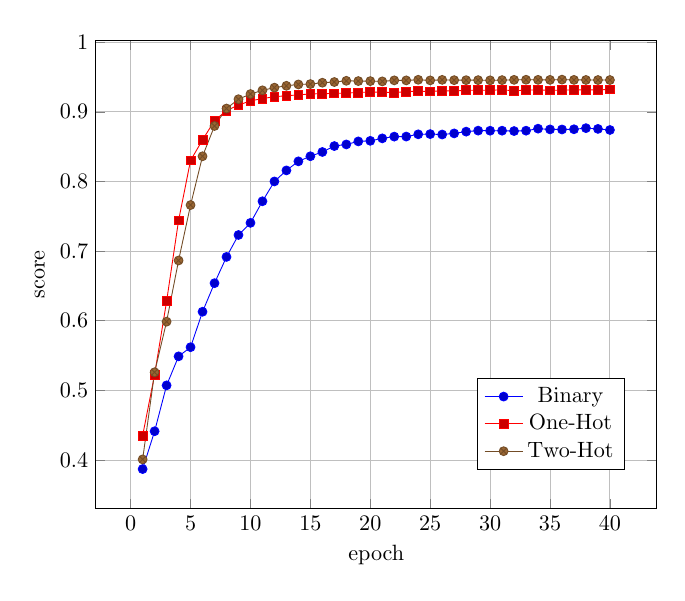
\begin{tikzpicture}[scale=0.8]
	\begin{axis}[
		height=9cm,
		width=9cm,
		grid=major,
        xlabel={epoch},
        ylabel={score},
        %every axis y label/.style= {at={( 0.1, 1.1)}, anchor=north},
        legend style={at={(0.68, 0.18)},anchor=west},
        x post scale=1.2
	]
		
	\addplot coordinates {
    (1, 0.38695000000000007)
    (2, 0.4412833333333333)
    (3, 0.50715)
    (4, 0.5488)
    (5, 0.5619833333333333)
    (6, 0.6128833333333333)
    (7, 0.6539166666666666)
    (8, 0.6916166666666665)
    (9, 0.7231166666666665)
    (10, 0.7405166666666667)
    (11, 0.7715666666666666)
    (12, 0.7999999999999999)
    (13, 0.8158500000000001)
    (14, 0.8288666666666668)
    (15, 0.8361999999999999)
    (16, 0.8422999999999999)
    (17, 0.8508333333333332)
    (18, 0.85315)
    (19, 0.8575166666666667)
    (20, 0.8583333333333334)
    (21, 0.8618833333333334)
    (22, 0.8644)
    (23, 0.8644666666666666)
    (24, 0.8676833333333334)
    (25, 0.868)
    (26, 0.8674)
    (27, 0.8690000000000001)
    (28, 0.8715333333333334)
    (29, 0.8729666666666667)
    (30, 0.87285)
    (31, 0.8728833333333333)
    (32, 0.8723666666666667)
    (33, 0.8729)
    (34, 0.8758)
    (35, 0.87475)
    (36, 0.87465)
    (37, 0.87495)
    (38, 0.8765333333333333)
    (39, 0.8754666666666666)
    (40, 0.8739166666666667)
    };
	\addlegendentry{Binary}

    % \addplot[color]
	\addplot coordinates {
    (1, 0.43484999999999996)
    (2, 0.5227)
    (3, 0.6278333333333334)
    (4, 0.7440333333333333)
    (5, 0.8301833333333333)
    (6, 0.8596666666666666)
    (7, 0.8873666666666667)
    (8, 0.9018333333333333)
    (9, 0.9097333333333332)
    (10, 0.9156833333333333)
    (11, 0.9189833333333334)
    (12, 0.9217000000000001)
    (13, 0.9230666666666666)
    (14, 0.92435)
    (15, 0.9256500000000001)
    (16, 0.9261333333333335)
    (17, 0.9263166666666666)
    (18, 0.9270166666666667)
    (19, 0.9276999999999999)
    (20, 0.9285166666666665)
    (21, 0.9281166666666666)
    (22, 0.9275666666666668)
    (23, 0.9290333333333333)
    (24, 0.92965)
    (25, 0.9292000000000001)
    (26, 0.9302333333333332)
    (27, 0.9299333333333332)
    (28, 0.9308500000000001)
    (29, 0.9310333333333333)
    (30, 0.9309833333333333)
    (31, 0.9315666666666665)
    (32, 0.9302)
    (33, 0.9311833333333334)
    (34, 0.93145)
    (35, 0.9307666666666666)
    (36, 0.9310999999999999)
    (37, 0.9316333333333334)
    (38, 0.9314166666666667)
    (39, 0.9314999999999999)
    (40, 0.9321)


	};

	\addlegendentry{One-Hot}
    
    
	\addplot coordinates {
    (1, 0.40083333 )
    (2, 0.52598333 )
    (3, 0.59866667 )
    (4, 0.6865     )
    (5, 0.7661     )
    (6, 0.83616667 )
    (7, 0.87966667 )
    (8, 0.90473333 )
    (9, 0.91811667 )
    (10,0.92553333 )
    (11,0.93085    )
    (12,0.93471667 )
    (13,0.93736667 )
    (14,0.93931667 )
    (15,0.93986667 )
    (16,0.94178333 )
    (17,0.94278333 )
    (18,0.94453333 )
    (19,0.94416667 )
    (20,0.94411667 )
    (21,0.94368333 )
    (22,0.94518333 )
    (23,0.94515    )
    (24,0.946      )
    (25,0.94515    )
    (26,0.94588333 )
    (27,0.94546667 )
    (28,0.94545    )
    (29,0.9455     )
    (30,0.94523333 )
    (31,0.94553333 )
    (32,0.94591667 )
    (33,0.94605    )
    (34,0.94591667 )
    (35,0.94588333 )
    (36,0.9462     )
    (37,0.94585    )
    (38,0.94576667 )
    (39,0.94565    )
    (40,0.94566667 )


    };
	\addlegendentry{Two-Hot}
    
	\end{axis}
\end{tikzpicture}


\captionof{figure}{Each point in this chart is the average of the validation
accuracy on the best models at epoch $i$; we have performed the same process
three times by changing  one factor, the encoding.}
\label{comparingEnc}
\end{center}


\subsubsection{Diacritics}
% NOTE: refine it.
 Diacritics give more information about the pattern. On average, diacritic models
outperforms the no-diacritic models, but from the result table \ref{ar-results},
model 1 and 2 which are Two-Hot diacritic and no-diacritic, respectively, reached
the same results. But in other encoding methods, diacritic models outperforms the
no-diacritic models.







  
%In general, two-hot encoding performs better than the binary encoding and has a steeper learning curve.  In big archicture with unwieghted models, binary encoding results were close to the two-hot results, but the two-hot is still better.  
\subsection*{Imbalanced Dataset effect}
As char \ref{data_size} shows, the dataset is imbalanced, big classes have enough
data to train the model well, while small classes do not; small classes' size is
less than 18,000 data points. To handle this situation we have presented two
methods: weighting the loss function and eliminating the small classes. For
weighting the loss function, it does not effect the results as we previously
thought. The following table contains 4 models.

\begin{center}
\begin{tabular}{|c|c|c||c|c|} 
\hline
Class & Model 1 & Model 2 & Model 3 & Model 4\\ 
\hline
% Model 1:
% 94.5%
% relearn_drop_2_Exp_6_full_data_matrix_without_tashkeel_two_hot_encoding_Bidirectional_LSTM_6_50_1

% Model 2:
% 95.43%
% Model 2: % relearn_drop_2_Exp_6_full_data_matrix_without_tashkeel_two_hot_encoding_Bidirectional_LSTM_6_50_0

% Model 3: 
% 95.51%
% relearn_drop_2_Exp_7_full_data_matrix_with_tashkeel_8bitsEncoding_Bidirectional_LSTM_6_81_0

% Model 4:
% 94.6%
% relearn_drop_2_Exp_7_full_data_matrix_with_tashkeel_8bitsEncoding_Bidirectional_LSTM_6_81_1
   Wafeer    &   94.64\%   &  95.98\%    &  96.19\%   &  95.76\%  \\
   Monsareh  &   86.79\%   &  89.48\%    &  90.32\%   &  88.7\%  \\
   Madeed    &   78.01\%   &  81.28\%    &  82.79\%   &  81.78\%  \\
   Mogtath   &   80.09\%   &  84.53\%    &  87.77\%   &  83.76\%  \\
   Motakarib &   94.18\%   &  96   \%    &  95.1 \%   &  94\%  \\
   Kamel     &   95.74\%   &  96.74\%    &  96.37\%   &  95.84\%  \\
   Taweel    &   97.61\%   &  97.81\%    &  98.29\%   &  97.27\%  \\
   Sar'e     &   86.73\%   &  90.18\%    &  91.1 \%   &  90.33\%  \\
   Raml      &   92.54\%   &  92.98\%    &  92.79\%   &  91.13\%  \\
   Rigz      &   85.23\%   &  86.11\%    &  85.8 \%   &  83.22\%  \\
   Khafeef   &   95.58\%   &  96.59\%    &  96.63\%   &  96.24\%  \\
   Baseet    &   97.64\%   &  98.03\%    &  97.97\%   &  97.63\%  \\
   Moktadib  &   52.04\%   &  68.36\%    &  62.24\%   &  59.81\%  \\
   Hazg      &   78.57\%   &  77.79\%    &  78.31\%   &  72.73\%  \\
   Modar'e   &   0         &  20.83\%    &  33.33\%   &  16.67\%  \\
   Motadarik &   70.67\%   &  78.86\%    &  77.52\%   &  78.48\%  \\
\hline
\end{tabular}
\captionof{table}{Model 1 and 2 share the same architecture (7 layer, 50 units)
but the model 1's loss function is weighted and model 2's is not. Also, model 3
and 2's architecture is (7 layers, 81 units), model 3's loss function is wieghted
and model 4's is not.}
\end{center}


  
The second method, is to eliminate the small classes, the eliminating purpose is
not balancing the dataset; but our purpose is to study the effect of existing
such the small classes on the performance. We have noticed that eliminated
method needs at least 82 units so that it increases the accuracy.

% NOTE: Elemenating the small classes increase the accuracy for unweighted.
% NOTE: Elemenated becomes better with more units.
% NOTE: Full need deeper network.


% In eliminated unweighted without-diacritic case, in which each class has enough
% data to learn from, binary encoding results has reached the two-hot encoding
% results but with a more complex architecture than the two-hot, and this shows
% that if there is enough data for each class, binary unweighted without-diacritic
% models will result in high performance but with more complex architecture. We
% think that two-hot encoding outperforms the binary encoding because of the
% common feature problem which is previously presented.
% NOTE: add ref to the common feature problem.

% On average, full data unweighted models has better results than the full data
% weighted models. But eliminated data weighted and eliminated data unweighted
% models has so close results, this means that the weighted loss does not effect.







%%%%%
\subsection*{English Results}
\begin{center}
 \begin{tabular}{c c c c} 
     %\hline
     \toprule
     \textbf{id} & \textbf{encoding } & \textbf{cell type} & \textbf{f1 test}\\
     %\hline
     \midrule
     1 & one-hot & GRU  & 81.35\%\\ % exp69
%     2 & one-hot & GRU  & 79.49\%\\ % exp45
     2 & one-hot & LSTM & 80.34\%\\ % exp88
%     4 & binary  & GRU  & 73.52\%\\ % exp89
     3 & binary  & LSTM & 75.43\%\\ % exp46
     4 & binary  & GRU  & 75.04\%\\ % exp90

     %\hline
     \bottomrule
 \end{tabular}
\captionof{table}{Best performance models}
\label{eng-results}
\end{center}

% NOTE: add that the dataset is relatively small.

% Best Performance
Generally, GRU models outperform LSTM and Bi-LSTM models.  The model which shows
the highest performance is in the experiment 1 in the previous table, f1 =
0.8135. The model consists of 7 hidden layers, 40 units per each layer, 0.1
dropout and 128 batch size. 

% Encoding effect
On average, the highest results are achieved by the one-hot representation not by
the binary; this is because in one-hot encoding each character is represented by
a one-hot vector which have no common features between letters, this is not the case in
the binary encoding, in which each letter is represented by a unique binary
combination, so each letter may share some common features in its representation
with the others, which in turn confuses the model, it needs more complex and
deeper network to achieve results similar to what one-hot achieves due to the
common feature problem
\ref{commonFproblem}.
% NOTE:
% GRU performs better with one-hot as it is shown in experiments 1, 2
% and also, LSTM performs better with one-hot as experiments 3, 4 shows.

% NOTE: architrave effect and NOTE. 


% SOME NOTES
\begin{center}
    \small
    \begin{tabular}{ *{5}{E}}
        \woB{} & \woB{Iambic}   & \woB{Anapaestic} & \woB{Trochaic} & \woB{Dactyle}\\
        \woB{Iambic}     & 0.8998 & 0.045  & 0.0529  & 0.00189 \\
        \woB{Anapaestic} & 0.0919 & 0.884  & 0.01838 & 0.00551 \\
        \woB{Trochaic} 	 & 0.34   & 0.0375 & 0.6196  & 0       \\
        \woB{Dactyle}    & 0      & 0.014  & 0       & 0.9859  \\
    \end{tabular}
\captionof{table}{The best model's confusion matrix}
\end{center}
The above confusion matrix is of the best model, experiment 1 in the table
\ref{eng-results}, which we have presented in
the beginning of this section. Row are the real classes and columns are the
predictions.  There are some notes we can derive from it like; \textit{Dactyl}
class is hardly misclassified whether false-positive or false-negative; this
is because \textit{Dactyl} verses are hexameter which is relatively longer than
the three remaining classes, they are pentameter or less; so usually any long
verse is classified as \textit{Dactyl}. To study the that case, we have dropped
the relatively long-verse \textit{Dactyl} and trained the best model (experiment
1), we have got f1=78.8\%, which is less than the experiment 1 f1, this is
because of the lack of data. Our English dataset is so small, as it discussed in
the dataset section.

% NOTE: add we need more data.
% while one sweet smile gives patrick the wealth of a nation; anapestic
% is misclassified as dactyl, because of most dactly are long.  


